% Optimization Project: Biscuit Optimizer
% Roberto Basla
% Politecnico di Milano
% A.Y. 2021/2022

\section{Heuristic solutions}\label{sec:heuristics}
As the solvers were not able to find a solution in a reasonable time, some heuristics were devised to tackle the problem. Python notebooks ot the experiments are available in the GitHub repository  \href{https://github.com/rb-sl/biscuit_optimizer/tree/main/src/03-heuristics}{rb-sl/biscuit\_optimizer/src/03-heuristics}.

\subsection{Greedy heuristics}\label{sec:greedy}
The first set of heuristics tries to solve the nesting problem greedily. In order to do so, a series of cost map encoding the cost of activating a variable \texttt{y[i, n, m]} (i.e., placing a cutter of type $i$ at coordinates $(n, m)$) was defined:
\begin{itemize}[itemsep=-1mm, topsep=0mm]
	\item Value-based cost map: assigns the cost $c_{i,n,m} = -v_i$ (i.e. the negative value of cutter $i$) to each \texttt{y[i, n, m]} independently of the position $(n, m)$
	\item Area-based cost map: assigns the cost $c_{i,n,m} = a_i$ (i.e. the area consumption of cutter $i$) to each \texttt{y[i, n, m]} independently of $(n, m)$
	\item Occupancy-based cost map: assigns to each \texttt{y[i, n, m]} a cost proportional to the number of \texttt{y} variables that would be made infeasible by activating \texttt{y[i, n, m]} at the first step, $c_{i, n, m} = \textrm{len}(o_{i, n, m})$ with $o$ representing the list of $y$s made infeasible by each $(i, n, m)$
	\item Composition of Value and Area cost maps: $c_{i, n, m} = -\frac{v_i}{a_i}$
	\item Composition of Value and Occupancy cost maps: $c_{i, n, m} = -\frac{v_i}{o_{i, n, m} + 1}$
	\item Composition of Area and Occupancy cost maps: $c_{i, n, m} = (o_{i, n, m} + 1) \cdot a_i$
\end{itemize}
These cost maps define the quantities to be minimized by the greedy procedures, while the actual results refer to the sum of biscuit values. 

\subsubsection{Results}
Heuristics were run 100 times to find average results for each strategy. Figure \ref{fig:heuristics_results} shows their distribution: only strategies involving the occupancy were consistent in their results, as that was the only cost map that defined values for $(i, n, m)$ instead of for $i$ only. Other heuristics had intrinsic randomness, either explicitly defined (as in the case of greedy/random) or implicitly (e.g., the area case would be greedy only in choosing the cutter and random in selecting the position).

Table \ref{tab:heuristics_results} reports average values and time for the simulations; it introduces a completely random baseline to compare the results. In general, results were worse than the ones provided by complete nesting models; in particular, heuristics including areas performed worse than the other cases (area-based only was even worst than the random baseline). The best performing strategy (greedy combining value and occupancy) is kept for the next section.

\begin{center}
	\begin{tabular}{r|c|c}
		Heuristic					& Average value	& Time for 100 simulations (s) 	\\
		\hline
		Random (baseline) 			& 9151 			& 277.8 						\\
		Greedy/Random 				& 13489 		& 331.79 						\\
		Greedy (value) 				& 13249			& 334.69 						\\
		Greedy (area) 				& 9000 			& 260.93						\\
		Greedy (occupancy) 			& 15600			& 329.51						\\
		Greedy (value+area) 		& 9555			& 258.44						\\
		Greedy (value+occupancy)	& 16900			& 353.11						\\
		Greedy (area+occupancy)		& 15600			& 378.72						\\
	\end{tabular}
	\captionof{table}{\label{tab:heuristics_results}Heuristics results}
\end{center}

\begin{figure}[H]
	\centering	
	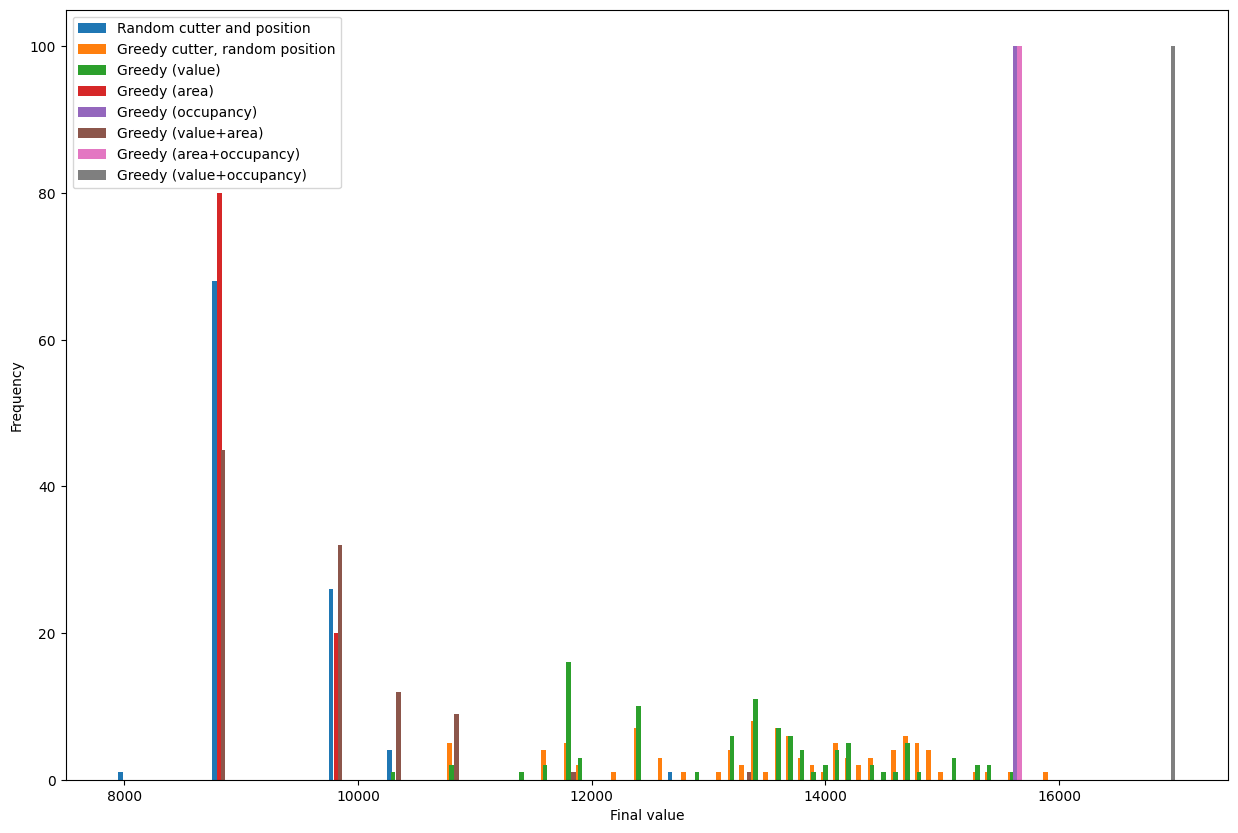
\includegraphics[width=\textwidth]{03-heuristics/heuristic_simulations}
	\caption{Distribution of heuristic results over 100 simulations for each strategy}
	\label{fig:heuristics_results}
\end{figure}

\subsection{GRASP}
The last class of implemented heuristics is Greedy Randomized Adaptive Search Procedures as described by Resende and Ribeiro\cite{grasp}. It is composed of two main phases that are iterated a number of times.

\paragraph{Greedy Randomized Construction} This phase builds a solution by first creating a Restricted Candidate List (RCL) containing elements with the smallest incremental cost as defined by the cost map. Elements $e = (i, n, m)$ are chosen to be part of the RCL if their cost $c(e)$ is
$$
c(e) \in [c^{min}, c^{min} + \alpha (c^{max} - c^{min})]
$$ 
For some choice of $\alpha$. The next element is chosen randomly from the RCL.

\paragraph{Local search} This phase searches the neighborhood of the solution found by the previous phase as in Hill Climbing. The neighborhoods are built according to the scheme defined by Delorme et al.\cite{local_search} using k-p exchanges, which consist in varying k variables from 1 to 0 and p variables from 0 to 1. In particular were used 0-1, 1-1, 1-2 and 2-1 exchanges.

\vspace{20px}

While previous heuristics encoded solutions as human-readable Python dictionaries, results are now 3D NumPy arrays of shape $n_{cutters} \times n_{rows} \times n_{columns}$ that correspond to variables $y$ in Section \ref{sec:nesting}:
\begin{equation}\notag
	y_{i, n, m} = 
	\begin{cases}
		1 \quad \textrm{if the solution has a cutter } i \textrm{ in position } (n, m) \\
		0 \quad \textrm{otherwise}
	\end{cases}
\end{equation}
With this definition, the symmetric distance becomes just
$$
\Delta(s, g) = \sum_{i \in I}\sum_{n \in N}\sum_{m \in M} |s_{i, n, m} - g_{i, n, m}|
$$
i.e. the number of different elements between the starting solution $s$ and the guiding solution $g$.

This project's implementation made some changes with respect to the paper's description, namely:
\begin{itemize}[itemsep=-1mm, topsep=0mm]
	\item The Greedy Randomized Construction phase doesn't stop in order to avoid impeding the construction of a feasible solution with the remaining cutters for performance purposes: this change improved the construction time to 2s from 21s (on average) without impacting the quality of solutions
	\item The Greedy Randomized Construction phase doesn't build infeasible solutions, so the repair procedure is not needed
	\item The Local Search uses two additional parameters limiting the maximum total time and the maximum time between improvements, as the neighborhood exploration is the slowest phase (even if it can be faster when starting from a good solution\cite{local_search})
\end{itemize}

\subsubsection{Path Relinking}
Path Relinking aims at exploring trajectories connecting solutions obtained by the GRASP procedure. It keeps an elite pool of the best solutions found and relinks them to new GRASP solutions, potentially obtaining better results. The choice of which (initial) solution is relinked to the other (guiding) determines the type of Path Relinking. This project implements the following alternatives, as described in \cite{grasp}:
\begin{itemize}[itemsep=-1mm, topsep=0mm]
	\item Forward Path Relinking: the GRASP output is the initial solution while the guiding solution is chosen from the elite pool according to its distance
	\item Backward Path Relinking: the roles of initial and guiding solutions are reversed with respect to the previous case
	\item Mixed Path Relinking: the origin of the two solution is changed at each iteration
	\item Evolutionary Path Relinking: every $e$ steps of any of the previous variants the solutions in the elite pool are relinked among themselves
\end{itemize}
The only changes with respect to the algorithm description in the paper were the addition of a tabu list to the local search phase containing the initial and guiding solutions (otherwise many solutions tend to fall back into local optima found by GRASP), and limiting the minimum distance of new elite solutions also when the pool is not full.

\subsubsection{Results}
GRASP and its Path Relinking variant were able to consistently reach and exceed the values obtained by nesting models of section \ref{sec:nesting}. Table \ref{tab:grasp_results} contains the best results for each of the implemented strategies.

\paragraph{GRASP} GRASP heuristics were run 100 times to assess the average value of solutions, which is close to that of the best heuristic in Section \ref{sec:greedy} (being 16834, obtained in 17315.07s). However, it was able to reach higher values as shown in Figure \ref{fig:grasp_100}, and considering that GRASP's result are actually given by the best one among a number of iterations (instead of just one as in the test), it is able to consistently outperform the previously considered heuristics. An example using 5 iterations is reported in Table \ref{tab:grasp_results}.

\paragraph{Path Relinking} Path Relinking proved to be a good enhancement: the following output shows an example where solutions with values 16900 and 17900 generated a solution with value 17400 (the best one along the path), which led to the best solution after local search.

\begin{footnotesize}
	\begin{verbatim}
		PATH RELINKING: 6/10
		GRASP: 1/3
		Starting local search from solution v=15900
		Best solution after local search (5 improvements / 13095 checked): v=16900
		GRASP: 2/3
		Starting local search from solution v=15300
		Best solution after local search (5 improvements / 19186 checked): v=16100
		GRASP: 3/3
		Starting local search from solution v=15400
		Best solution after local search (4 improvements / 18033 checked): v=16400
		>>> [17900, 17500, 17900, 17200, 17900]
		Starting relinking of solution v=16900 to v=17900 (distance = 40.0)
		Best relinking solution in path (40 steps / 328 checks): v=17400 at step=39
		Best solution after local search (2 improvements / 2335 checked): v=18300
	\end{verbatim}
\end{footnotesize}
An example of Path Relinking and Local Search is displayed in Figure \ref{fig:path_relinking}. This enhancement was not tested for 100 steps as the output is not independent from previous iterations. However, it was able to find a solution with value 18500 (shown in Figure \ref{fig:pr_18500}), performing better than the Python models. 

Finally, the following output shows an example of successful evolution, where the new elite pool consists in the result for \texttt{k=4}:
\begin{footnotesize}
	\begin{verbatim}
		k=1: [16800,17100,16900]             => [17300,16900,16800,17000,16600]
		k=2: [17300,16900,16800,17000,16600] => [17200,17500,17500,17600,17500]
		k=3: [17200,17500,17500,17600,17500] => [17900,17600,17800,17600,17500]
		k=4: [17900,17600,17800,17600,17500] => [17800,17900,17800,17800,17700]
	\end{verbatim}
\end{footnotesize}

\begin{figure}[p]
	\centering
	\begin{subfigure}[b]{.49\textwidth}
		\centering
		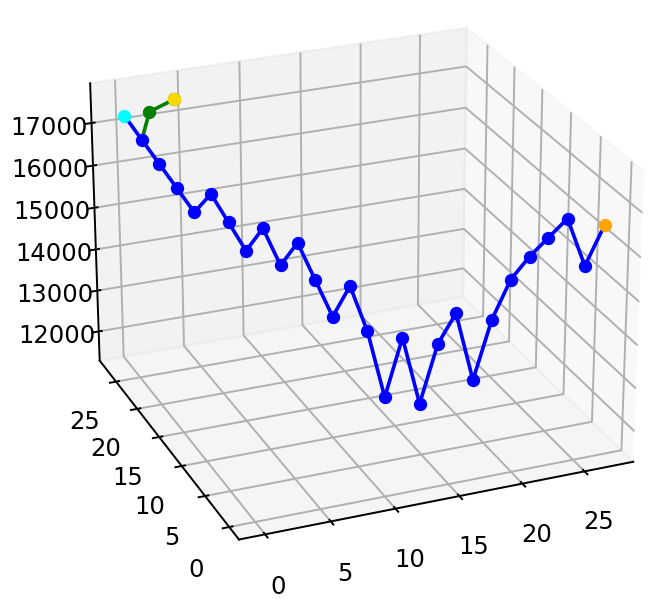
\includegraphics[width=\textwidth]{03-heuristics/paths/cut_pr_over}
		\caption{3D Path Relinking plot}
		\label{fig:pr_over}
	\end{subfigure}
	\hfill
	\begin{subfigure}[b]{.49\textwidth}
		\centering
		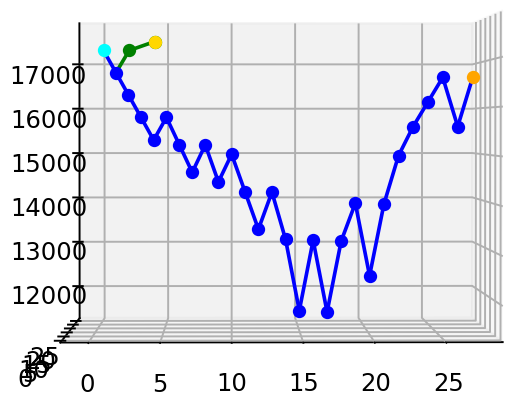
\includegraphics[width=\textwidth]{03-heuristics/paths/cut_pr_v_start}
		\caption{Projection over distance from the starting solution and value}
		\label{fig:pr_v_start}
	\end{subfigure}
	\caption{Path Relinking plot. Shows the starting solution (cyan), the guiding solution (orange) and the relinking path (blue). The Local Search path is in green, while the best final solution is gold. Axes correspond to distance from the starting solution, distance from the guiding solution and value.}
	\label{fig:path_relinking}
\end{figure}

\begin{figure}[p]
	\centering
	\begin{subfigure}[b]{.49\textwidth}
		\centering
		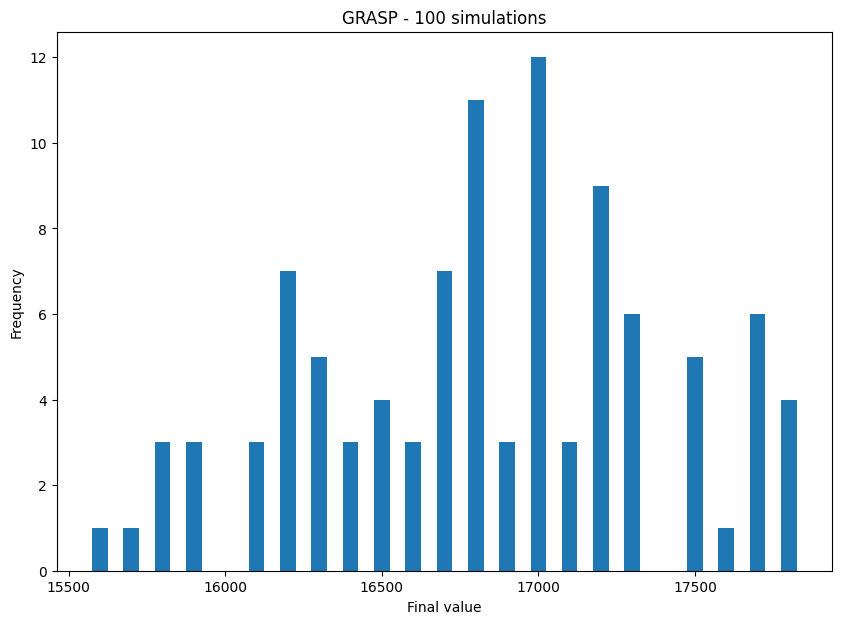
\includegraphics[width=\textwidth]{03-heuristics/grasp_100}
		\caption{100 single GRASP iterations}
		\label{fig:grasp_100}
	\end{subfigure}
	\hfill
	\begin{subfigure}[b]{.49\textwidth}
		\centering
		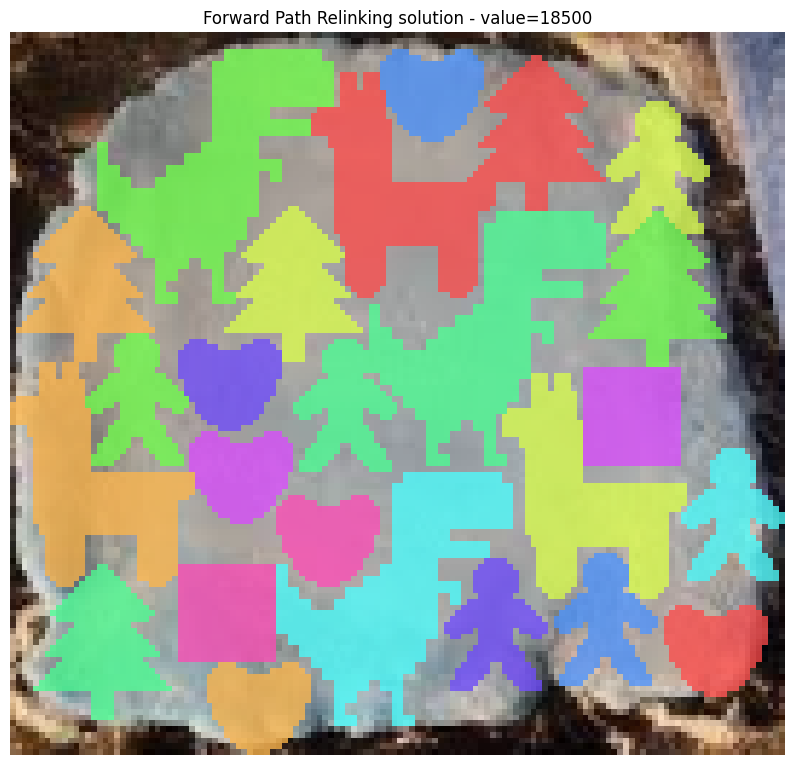
\includegraphics[width=\textwidth]{03-heuristics/pr_18500}
		\caption{Best Path Relinking solution}
		\label{fig:pr_18500}
	\end{subfigure}
	\label{fig:grasp_results}
	\caption{GRASP results}
\end{figure}

\vspace{20px}

\begin{center}
	\begin{tabular}{r|c|c|c}
		Heuristic							& Best value	& Iterations	& Time (s)	\\
		\hline
		GRASP 								& 17800			& 5				& 317.77	\\
		Forward Path Relinking				& 18500 		& 10 			& 2765.12	\\
		Backward Path Relinking				& 18300			& 10  			& 2761.82	\\
		Mixed Path Relinking 				& 18300			& 10	 		& 2776.01	\\
		Evolutionary Mixed Path Relinking	& 18300			& 20			& 9687.86	\\
	\end{tabular}
	\captionof{table}{\label{tab:grasp_results}GRASP and Path Relinking results}
\end{center}
